%\newcommand*{\thead}[1]{\multicolumn{1}{|l|}{\bfseries #1}}
\def\arraystretch{1.4}
\definecolor{tableHeader}{RGB}{211, 127, 47}
\definecolor{myOrange}{RGB}{255, 230, 210}
\newcolumntype{x}[1]{>{\centering\arraybackslash\hspace{0pt}}m{#1}}

\section{Planificació temporal}
	\label{sec:planificacio}
	El treball té una duració aproximada de 4 mesos i mig, des de setembre fins a principis de gener. La càrrega total serà d'unes 450 hores, corresponents a 18 crèdits ECTS.
	La dedicació setmanal estimada serà d'unes 25 hores.\\\\
	Es dividirà el projecte en quatre blocs, descrits a continuació:\\

	\begin{table}[H]
		\begin{center}
			\rowcolors{2}{myOrange}{white}
			\begin{tabular}{p{1.5cm} !{\vrule width -1pt}p{6cm} !{\vrule width -1pt}l !{\vrule width -1pt}l}
			\rowcolor{tableHeader}
			\textbf{Bloc} & \textbf{Descripció} & \textbf{Metodologia} & \textbf{Hores} \\
			Bloc 0 & Preparació de l'entorn & - & 5h \\
			Bloc 1 & Curs de GEP & Cascada & 75h \\
			Bloc 2 & Desenvolupament del projecte & Àgil & 340h \\
			Bloc 3 & Preparació de la defensa & - & 30h \\
			\end{tabular}
		\end{center}
		\caption{Blocs del projecte}
	\end{table}

	\subsection{Bloc 0: Preparació de l'entorn}
		Inicialment, s'instal·larà tot el programari necessari per començar a desenvolupar el projecte i es faran algunes proves bàsiques per familiaritzar-se amb el nou entorn de treball.
		Aquest primer bloc tindrà una durada aproximada de 5 hores.\\\\
		Per poder començar a treballar en el projecte, caldrà instal·lar:\\
		\begin{itemize}
			\item \textbf{Desenvolupament:} Python, OpenCV, Geany i Git.
			\item \textbf{Curs de GEP:} Gantt Project.
			\item \textbf{Documentació:} {\LaTeX} i Zathura.
		\end{itemize}

	\subsection{Bloc 1: Curs de GEP}
		Aquest bloc correspon a la realització del curs de GEP, amb inici el dia 19/09/2016 i finalització el 24/10/2016 (amb una presentació final entre el 7 i l'11 de novembre).
		Té com a dependència el bloc 0.\\\\
		Durant el curs s'entregaran 6 lliurables, detallats a continuació:\\
		\begin{table}[H]
			\begin{center}
				\rowcolors{2}{myOrange}{white}
				\begin{tabular}{p{5cm} !{\vrule width -1pt}x{2.1cm} !{\vrule width -1pt}x{2.4cm} !{\vrule width -1pt}x{1.6cm} !{\vrule width -1pt}x{1.6cm}}
				\rowcolor{tableHeader}
				\textbf{Descripció} & \textbf{Inici} & \textbf{Finalització} & \textbf{Durada} & \textbf{Hores} \\
				Introducció i abast & 19/09/2016 & 27/09/2016 & 9 dies & 16h \\
				Planificació temporal & 28/09/2016 & 03/10/2016 & 6 dies & 9h \\
				Gestió econòmica i sostenibilitat & 04/10/2016 & 10/10/2016 & 7 dies & 10h \\
				Presentació preliminar en vídeo & 11/10/2016 & 17/10/2016 & 7 dies & 11h \\
				Plec de condicions & 18/10/2016 & 24/10/2016 & 7 dies & 13h \\
				Document final + presentació & 18/10/2016 & 24/10/2016 & 7 dies & 16h
				\end{tabular}
			\end{center}
			\caption{Lliurables de GEP}
		\end{table}

	\subsection{Bloc 2: Desenvolupament del projecte}
			El bloc principal consistirà en el desenvolupament del projecte en si mateix: buscar informació, implementar el codi, redactar la memòria, etc.\\\\
			Aquest bloc té com a dependència el bloc 0 i es dividirà en quatre tasques.\\
			\begin{table}[H]
				\begin{center}
					\rowcolors{2}{myOrange}{white}
					\begin{tabular}{p{5cm} !{\vrule width -1pt}x{2.1cm} !{\vrule width -1pt}x{2.4cm} !{\vrule width -1pt}x{1.6cm} !{\vrule width -1pt}x{1.6cm}}
					\rowcolor{tableHeader}
					\textbf{Tasca} & \textbf{Inici} & \textbf{Finalització} & \textbf{Durada} & \textbf{Hores} \\
					Implementació i proves & 13/09/2016 & 19/12/2016 & 98 dies & 240h \\
					Conclusions i resultats & 20/12/2016 & 31/12/2016 & 12 dies & 30h \\
					Ampliacions (opcional) & 01/01/2017 & 09/01/2017 & 9 dies & 30h \\
					Redacció de la memòria & 10/10/2016 & 09/01/2016 & 92 dies & 40h \\
					\end{tabular}
				\end{center}
				\caption{Tasques desenvolupament}
			\end{table}

		\subsubsection{Recerca d'informació, implementació i proves}
			Una part molt important del projecte serà la cerca d'informació i l'estudi de les diverses eines i algorismes a utilitzar (com per exemple OpenCV i les seves funcions).
			Se cercarà informació contínuament i s'aniran fent proves a mesura que s'implementa el codi.\\\\
			La fase d'implementació es dividirà en diverses tasques, que s'aniràn realitzant a mesura que avanci el projecte. Algunes d'aquestes tasques seràn:
			\begin{itemize}
				\item{Obtenció de keypoints (Harris)}
				\item{Extracció de característiques (SIFT)}
				\item{Matching i homografia}
				\item{Altres algorismes (ORB, BRISK, BRIEF)}
				\item{Disseny de l'aplicació d'Android}
				\item{Creació de l'aplicació d'Android}
			\end{itemize}
		\subsubsection{Conclusions i resultats}
			Un cop enllestida la implementació, es procedirà a elaborar les conclusions d'acord amb els resultats obtinguts. Es compararan els resultats obtinguts amb diferents algorismes de visió i es faran
			proves del sistema amb diverses imatges.
		\subsubsection{Ampliacions (opcional)}
			Un cop realitzades les conclusions, en cas de disposar de més temps, es podran fer ampliacions i millores.\\\\
			En cas de patir un retard en la planificació del projecte, s'utilitzarà aquest temps per acabar l'etapa de les conclusions.
		\subsubsection{Redacció de la memòria}
			La memòria s'anirà redactant a mesura que es realitza el projecte. No hi ha per tant cap dependència, encara que es dedicarà més temps en l'etapa final del treball.\\

	\subsection{Bloc 3: Preparació de la defensa}
	En aquest bloc final es revisarà la memòria del projecte i es prepararà la presentació. Està previst dedicar unes 30 hores al bloc, que començarà el dia 10 de gener i acabarà el 22.
	La defensa del projecte es durà a terme entre els dies 23 i 27 de gener.

	\subsection{Diagrames}
		%Durant la fase de planificació del projecte, s'han realitzat diversos diagrames. Podeu trobar tots aquests diagrames (Gantt i PERT) a l'apèndix \ref{appendix:diagrames} del treball.
		Durant la fase de planificació del treball, s'han realitzat diversos diagrames. A continuació podeu trobar els diagrames de PERT i el Gantt del projecte.\\

		\begin{figure}[H]
			\centering
			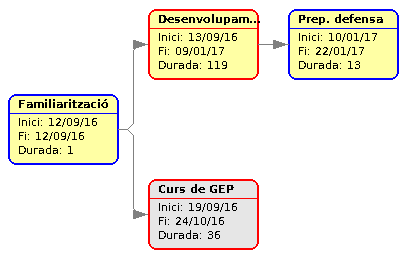
\includegraphics[width=0.7\textwidth]{images/pert-global}
			\caption{PERT del projecte}
		\end{figure}
		\vspace{0.8cm}
		\begin{figure}[H]
			\centering
			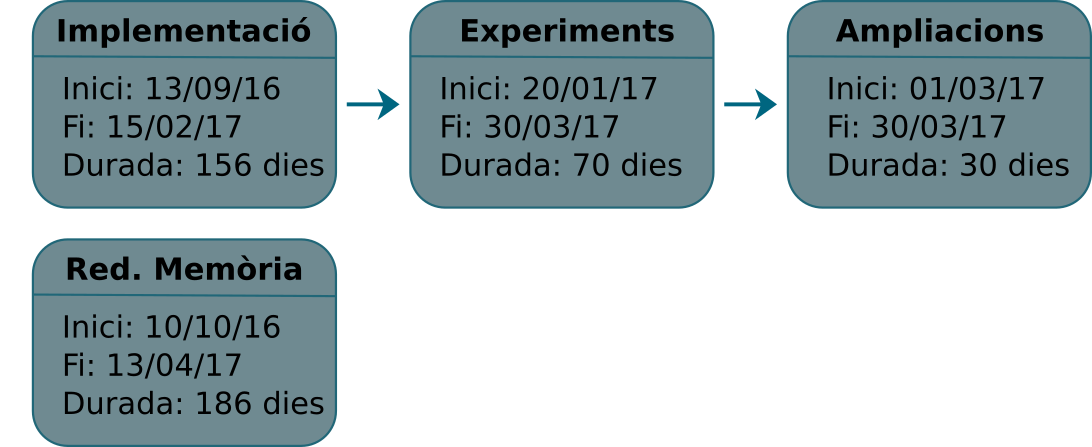
\includegraphics[width=0.7\textwidth]{images/tasques}
			\caption{PERT - tasques desenvolupament}
		\end{figure}

		\restoregeometry
		\newgeometry{bottom=1cm, top=1cm}
		\thispagestyle{empty}
		\begin{sidewaysfigure}
			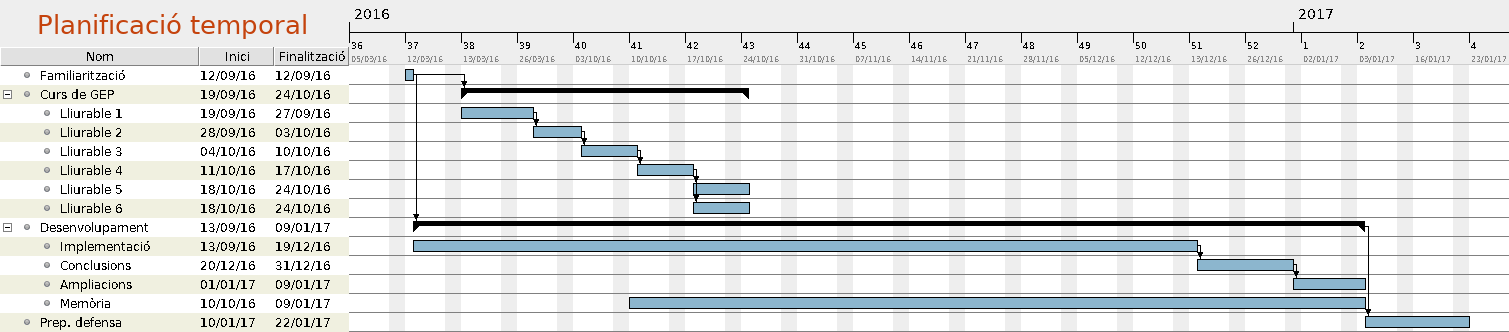
\includegraphics[width=\textheight]{images/gantt}
			\caption{Gantt del projecte}
		\end{sidewaysfigure}
		\restoregeometry
		\newgeometry{bottom=4.5cm}

\section{Recursos}
	En aquesta secció s'analitzen els recursos necessaris per a la realització del projecte. %A continuació es detallen els recursos humans, de maquinari i de programari utilizats.
	\subsection{Recursos humans}
		El projecte el realitzarà una sola persona, que haurà d'assumir els rols de cap de projecte, analista, dissenyador, programador i \textit{tester}.
		També es comptarà amb l'ajuda del director del projecte, que assumirà el paper de consultor/supervisor.
	\subsection{Recursos de maquinari}
		Per la realització del projecte no serà necessari adquirir cap mena de maquinari específic. Es podrà utilitzar un ordinador personal per treballar a casa i els ordinadors disponibles a la FIB per
		treballar des de la universitat.\\\\
		Es treballarà principalment amb un ordinador equipat amb un processador AMD FX 6300 hexa-core 3.5GHz, 4GB de RAM i 250GB de disc dur SSD. També s'utilitzarà una càmera o smartphone qualsevol.
	\subsection{Recursos de programari}
	Durant la realització del projecte i el curs de GEP, s'utilitzaran diverses eines de programari, detallades a continuació:\\
	\begin{table}[H]
		\begin{center}
			\rowcolors{2}{myOrange}{white}
			\begin{tabular}{l !{\vrule width -1pt}p{5cm} !{\vrule width -1pt}p{5cm}}
			\rowcolor{tableHeader}
			\textbf{Nom} & \textbf{Tipus} & \textbf{Ús} \\
			Arch Linux & Eina de desenvolupament & Execució del programari \\
			Python & Eina de desenvolupament & Programació \\
			OpenCV & Eina de desenvolupament & Algorismes de VC \\
			Geany & Eina de desenvolupament & Programació del codi \\
			Android Studio & Eina de desenvolupament & Programació del codi \\
			Gimp/Inkscape & Eina de desenvolupament & Retocs i creació d'imatges \\
			\LaTeX & Eina de desenvolupament & Redacció de la memòria \\
			Zathura & Eina de desenvolupament & Visualització de pdf \\
			Gantt Project & Eina de gestió & Creació diagrames de Gantt \\
			LibreOffice Calc & Eina de gestió & Control de les hores \\
			Git + Github & Desenvolupament i gestió & Control de versions \\
			\end{tabular}
		\end{center}
		\caption{Recursos de programari}
		\label{table:programari}
	\end{table}
	
\section{Desviacions i pla d'actuació}
	\subsubsection{Mala planificació [Impacte: baix]}
		Hi haurà reunions amb el director i s'usaran eines de planificació per mirar de corregir la planificació i acabar el projecte a temps. També es reserven unes hores a l'ampliació del treball,
		que es podrien utilitzar en cas que una tasca s'allargués més del previst. Si fos necessari, es podria incrementar una mica la càrrega de treball setmanal.
	\subsubsection{Fallades de maquinari [Impacte: baix]}
		En cas de fallades en l'ordinador principal, no hi hauria cap problema en utilitzar-ne un altre. No hi ha dependències de hardware i es disposa d'altres ordinadors (a casa i a la FIB).
		Tampoc hi hauria una pèrdua de dades important, ja que es treballa amb Github i una còpia local.
